% This is samplepaper.tex, a sample chapter demonstrating the
% LLNCS macro package for Springer Computer Science proceedings;
% Version 2.20 of 2017/10/04
%
\documentclass[runningheads]{llncs}
%
\usepackage{graphicx}
% Used for displaying a sample figure. If possible, figure files should
% be included in EPS format.
%
% If you use the hyperref package, please uncomment the following line
% to display URLs in blue roman font according to Springer's eBook style:
% \renewcommand\UrlFont{\color{blue}\rmfamily}
\begin{document}
%
\title{Delay Analysis for URLLC in 5G Based on Stochastic Network Calculus\thanks{Supported by program National Natural Science Foundation of China. (Nos.61370065,61502040).
Beijing Municipal Program for Excellent Teacher Promotion. (No.PXM2017\_014224.000028).}}
%
%\titlerunning{Abbreviated paper title}
% If the paper title is too long for the running head, you can set
% an abbreviated paper title here
%
\author{Shengcheng Ma\inst{1}\orcidID{0000-0003-1060-1208} \and
Zhuo Li\inst{1}\orcidID{1111-2222-3333-4444} \and
Xin Chen\inst{1}\orcidID{2222--3333-4444-5555}}
%
\authorrunning{SC Ma et al.}
% First names are abbreviated in the running head.
% If there are more than two authors, 'et al.' is used.
%
\institute{Beijing Information Science and Technology University, Beijing 08544, China \and
Springer Heidelberg, Tiergartenstr. 17, 69121 Heidelberg, Germany
\email{mashengcheng@163.com}\\
\url{http://www.springer.com/gp/computer-science/lncs} \and
ABC Institute, Rupert-Karls-University Heidelberg, Heidelberg, Germany\\
\email{\{abc,lncs\}@uni-heidelberg.de}}
%
\maketitle              % typeset the header of the contribution
%
\begin{abstract}
The fifth generation (5G) wireless networks are upcoming to our life.
The higher performance requirements are raised to satisfy the needs in modern communication.
Ultra-reliable low latency communications (URLLC) is one of the most important scenarios in 5G.
URLLC with strict latency and reliability requirements is widely used in some delay-sensitive applications such as self-driving.
As the 3GPP claimed, the URLLC is amenable to 99.999\% transmission correctness and within 1ms delay bound.
How to meet the requirements of reliability and latency is still an open issue.
Some academic studies and companies proposed various methods to design URLLC standard, but little effort has been made on applying a theoretical method to analyze the delay bound.
Stochastic network calculus is an elegant way to obtain the delay bound based on traffic models and service guarantees.
In this paper, we take the character of 5G architecture into account and use the stochastic network calculus to analyze the delay in URLLC.
Some factors which can influence on the delay are obtained.
Optimizing these factors to reduce the delay will provide valuable guidelines for the early design of URLLC architecture.
Finally, numerical results are presented to verify the correctness of the delay analysis.

\keywords{5G \and URLLC \and Stochastic Network Calculus \and Delay Analysis.}
\end{abstract}
%
%
%
\section{Introduction}
The 5G era is getting closer to us.
5G communication technology appeared for the first time with the 2018 Pyeongchang Winter Olympics in South Korea.
It helps audiences watch the live broadcast continuously and smoothly.
According to International Telecommunication Union announced the 5G standard timetable, 5G will start commercially in 2020 \cite{standard1}.
5G wireless networks are designed to support diverse and complicated scenarios.
The third generation partnership project (3GPP) classify these different scenarios into three big categories: enhanced mobile broadband (eMBB), massive machine type communications (mMTC), and ultra-reliable low-latency communications (URLLC) \cite{standard2}.

URLLC is widely used in self-driving, mission critical application and some delay sensitive systems.
It has stringent requirements in terms of delay and reliability in the 5G New Radio (NR) systems.
The key requirements of URLLC as claimed by the 3GPP are to ensure the latency of user plane data less than 1ms for downlink and uplink, meanwhile to keep very high packet reception reliability about 99.999 percent.\cite{article1}
The stringent delay requirement needs new 5G NR technology to bridge the gap.
Though the existing LTE networks can reach the reliability target, but the cost is some dozens of milliseconds time delay.
That is far away from the criteria of URLLC.
So the delay becomes the chock point and it needs to be solved.
Many academies and companies have proposed some engineering solutions to minimize the delay.
Such as the HARQ retransmission or grant-free technology.
However, how to analyze the generation of time-delay from a theoretical perspective and propose a strategy to reduce the delay effectively is an important research subject.

Stochastic network calculus (SNC) theory is very good at delay performance analysis.
The SNC is a continuous development method to analyze network traffic characteristic and evaluate performance\cite{book1}.
Different from queuing theory, the SNC permits some packets violate the desired performance.
This feature can better take advantage of statistical multiplexing gains\cite{article2}.
To deal with random service and statistical guarantee, the SNC theory comes into being with a large number of stochastic processes and network traffic models.
Under a suitable traffic model and a chosen server model, the SNC theory can process service guarantee analysis of communication network like delay and backlog.
So we capitalize on the SNC method to analyze the delay of the 5G URLLC transmission in this paper.

We use stochastic arrival curve to describe the process that user equipment (UE) data sends to gNodeB (gNB) side.
According to the 5G network topology architecture, we can deduce the rest stages of data transmission from gNB to cloud server.
Every stage of stochastic arrival curve characterizes the delay property, therefore the whole delay of URLLC system is comprised by delays which generated from UE to cloud server.

Our main contributions of this paper can be summarized as follows:

1) We build a tandem model to simulate 5G network architecture. In this model, we can analog the data transmission in uplink or downlink from UE to cloud server. We use stochastic service process and concatenation property to analysis the latency.

2) Our analysis results represent which parameters are the key factors affecting the delay. By adjusting the key factors, we give a group of tactics to reduced the delay effectively.

3) Delay analysis and tactics for reducing latency have valuable theoretical guidance for the design of URLLC deployment. In order to meet stringent delay requirements, it provides guidelines for how to allocate resources.

The rest of this paper is organized as follows.
Section II summarizes related work of URLLC technology and stochastic network calculus.
We present a tandem network model to describe URLLC in Section III.
In particular, we illustrate the architecture of this system and analyze the causes of the delay in this section.
In section IV, we introduce the experimental environment and analyze the relationship between latency and main factors.
We conclude this paper in Section V.
Some theoretical proofs are given in appendix.

\section{Related Work}
Because the standard of URLLC has not been worked out, many researchers have put forward different solutions for the design of URLLC.

Dozens of researches are focus on how to design and implement URLLC to meet the performance requirements.
A design without intervention in the baseband/PHY layer for URLLC is to use interface diversity and integrate multiple communication interfaces.
Jimmy and his colleagues propose an analysis framework that combines traditional reliability models with technology-specific latency probability distributions\cite{article_interface}.
In this way, they can estimate the performance in terms of latency and reliability in such an integrated communication system.
To guarantee a low end-to-end delay with low jitter over combined internet and wireless interfaces, the article \cite{article_multiconnectivity} presents a new multiple-input multiple-output(MIMO) networked round trip time (RTT) skew control controller.
This controller's advantage is that it solves the data flow split problem at the controlling node.
Jaya Rao and Sophie Vrzic have propose an approach to adopt packet duplication (PD) method to satisfy the latency and reliability requirements\cite{article_PD}.
PD technology generates multiple instances and sends them simultaneously in multiple unrelated channels.
The receiver selects the best packet according to the channel condition in order to achieve better transmission reliability.
This PD technique can provide a cost-effective solution without increasing the complexity in the radio access network (RAN).

In terms of resource allocation and energy efficiency, there are also some researches on URLLC.
How the frequency resource will be allocated to the user to send data in URLLC scenario.
That is an interesting study which is plunged by Anand A and De Veciana G\cite{article_Anand}.
Based on the 5G standard technology Orthogonal Frequency Division Multiple Access (OFDMA), they build a One Shot Transmission model.
Adopting queuing theory analysis, they find out a result that a small bandwidth over a longer duration is better than a large swath of bandwidth for short duration in One Shot Transmission system.
Green energy saving is getting more and more attention.
The article \cite{article_Energy} provides a coordinated on-off switching scheme across a set of adjacent gNBs.
The gNBs share a sleep schedule among themselves.
If the gNBs have lower traffic and fewer connected UEs, they will be set to the OFF mode.
This On-Off mode is more energy-efficient than traditional mode on the premise of guaranteeing the time delay.

Because URLLC has strict requirements for delay and reliability, it is very meaningful to evaluate the performance of URLLC.
Joachim et al. provide an achievable latency bound evaluation in their article\cite{article_joachim}.
They compare the latencies for different configurations in 5G RAN transmission.
The configuration contains FDD, TDD, frequency numerologies and usage of slots.
According the analysis, a frequency with higher numerology can be used to reduce the latency.
An article derived from HUAWEI company proposes a grant-free mode uplink transmission mechanism\cite{proc_Huawei}.
Grant-free transmission grant dynamically without scheduling request.
This mode is poised to meet the reliability requirement of URLLC in uplink transmission.
By simulating random arriving from different numbers of active UEs, the reliability can be improved after adopting the grant-free mode with increasing retransmission.

In order to satisfy the key requirements including latency and reliability, some state-of-the-art solutions have been discussed in \cite{article_Achieving}\cite{article_Wireless}\cite{article_Introduction}\cite{article_Physical}.
These technologies contains fast HARQ retransmission, MIMO, beam forming, diversity interfaces, D2D communication, Ultra Density Network and so on.
Some of these technologies can be employed alone to promote the performance, and others need to be combined together to achieve better results.
They all mentioned the design of frame structures.
That because low latency and high reliability are contradictory.
This requires more flexible frequency and time division.

Stochastic network calculus is a very practical tool, and it has a good practical effect in performance analysis and theoretical boundary calculation.

In these teams, there are often cooperation. The document \cite{MF_jiang} is an article of cooperation between Fidler M and Yuming Jiang, which mainly applies SNC theory to analyze the delay boundary of multi-server systems. Jiang also collaborate with BUPT team to evaluate the delay performance in wireless-powered communication system\cite{beiyou_1}.

\section{System Model}
\subsection{URLLC Network Architecture}
We consider URLLC network as a concatenate system from UE to Cloud. We only consider the 5G standalone network situation.
The 4G LTE network is composed by UE, RRU (Radio Remote Unit), BBU (Building Base band Unit), the EPC (Evolved Packet Core) which is the LTE's core network, and end by cloud servers.

Different to the 4G LTE, 5G networks are composed by UE, gNB, NGC and Cloud.
The gNB contains three parts that are AAU (Active Antenna Unit), DU (Distributed Unit) and CU (Centralized Unit).
AAU takes the place of the original RRU and combines some physical layer processing functions of BBU.
The BBU function of 4G will be rebuilt into DU and CU in 5G.
CU provides the service convergence function in the access side. It focuses on the low real-time capabilities of the protocol stack and adopt a centralized deployment.
DU mainly provides data access function to the terminal, including radio frequency and partial signal processing. DU concentrate on the high real-time capabilities of the transport requirements and suit for a distributed deployment method.
The NGC (Next Generation Core Network) as Core Network in 5G replace the EPC. 5G NGC is based on SDN/NFV technology and designed to better fit the cloud platform.
The architecture is depicted as Fig.\ref{fig_architecture}.
\begin{figure*}[htbp]
\centering
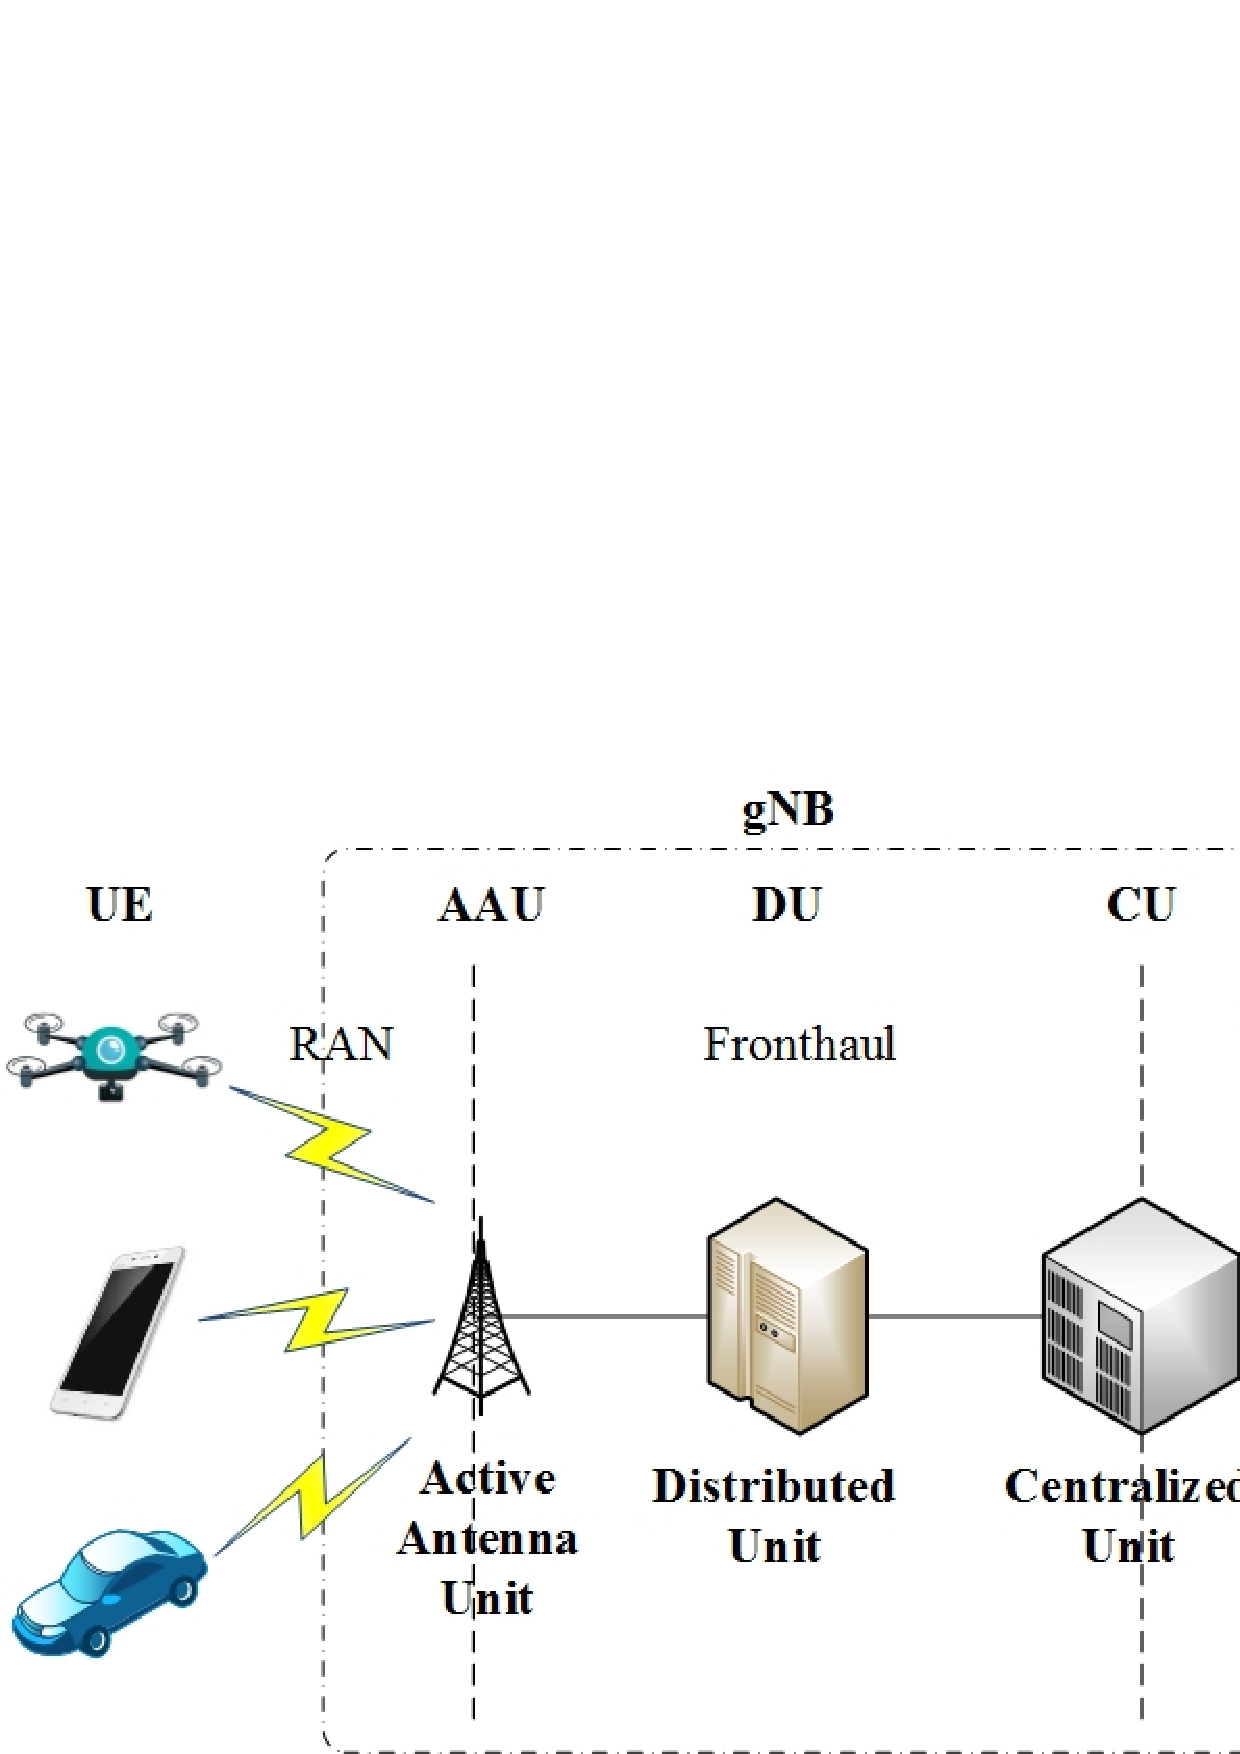
\includegraphics[width=\textwidth]{5G_delay_en.jpg}
\caption{5G network architecture.}
\label{fig_architecture}
\end{figure*}

\subsection{Delay of URLLC Network}
UE devices firstly access to AAU. The AAU is actually a part of base station. This part of the communication belongs to RAN.
UE's data will be accepted by AAU, and AAU put forward the data to DU.
There are two situations when data arrive at DU.
If CU and DU are deployed together, the data can be arrived at CU immediately. Otherwise, the data will be sent to CU from DU.
The communication from AAU to CU belongs to fronthaul.
The data leave CU and continue upward to the NGC. This part of the communication is called hackhaul.
NGC will process the data and it will take some time.
Finally, NGC sends the data to Cloud servers. The unidirectional transmission is finished.

So the whole delay or latency in 5G system is contribute by the time processing of RAN, fronthual, backhaul, Core Network and Cloud server. It can be expressed as Formula.\ref{eq_urllc_delay_composition}.
\begin{equation}\label{eq_urllc_delay_composition}
T_{Total} = T_{RAN} + T_{Fronthaul} + T_{Backhaul} + T_{NGC} + T_{Cloud}
\end{equation}
where
\begin{itemize}
\item $T_{RAN}$ is the time cost by physical layer transmission between UEs and AAU.
\item $T_{Fronthaul}$ is the delay between AAU to CU. It is the time taken in gNB.
\item $T_{Backhaul}$ is the time taken to communication between gNB to NGC.
\item $T_{NGC}$ is the delay taken place in NGC.
\item $T_{Cloud}$ is the latency which data transmission between NGC and Cloud server.
\end{itemize}
To meet the URLLC key requirement, we should do a good job of studying $T_{Total}$.
In this part, we discuss the latency mainly on the User Plane (UP) rather than Control Plane (C-Plane).
That because most of latency is attributed to the UP.
UP latency is the communication time between UE and network nodes when transmission and reception of the data at the corresponding IP layer.
Whereas, the C-Plane latency is the time spend on radio resource allocating and state switching from idle to active.
Compared with UP latency, the C-Plane delay is tiny and can be ignored.
\subsection{Problem Description}
The data is transferred from UE, through each nodes, and finally to the cloud.
According to the requirement of URLLC, the reliability and random latency \cite{MF_Random} can be described as Formula.\ref{eq_urllc_delay_problem}:

\begin{equation}\label{eq_urllc_delay_problem}
P\{delay > d \} < \epsilon
\end{equation}

The delay should be within 1ms, so the $d < 1$, the unit is millisecond (ms).
Where $\epsilon$ is defined as a very small probability.
%Meanwhile the block error rate (BLER) must be 99.999\%.
%It means that the value of $\epsilon$ must be less than $1*10^{-5}$, (i.e. $1 - 1*10^{-5} = 0.99999$, It equals to BLER $99.999\%$).
The Formula.\ref{eq_urllc_delay_problem} represents the 5G URLLC network successfully transport data and satisfy the delay requirements.
%and reliability

\subsection{Stochastic Network Calculus}
In SNC theory, the min-plus algebra is applied to analyze queuing system.
Let $\mathcal{F}$ denotes the set of non-negative non-decreasing functions and $\mathcal{\bar{F}}$ denotes the set of non-negative non-increasing function.
We employ the cumulative process to represent amount of traffic flow.
Arrival process, departure process and service process are denoted as $A(t)$, $D(t)$, and $S(t)$ respectively.
For any $0 \leqslant s \leqslant t, A(0)=0, A(s,t) = A(t) - A(s)$, and practical significance of $A(t)$ is the cumulative arrival data at time $t$.
It same to the $D(t)$ and $S(t)$.
Some fundamental definitions of curve are well described in literature \cite{b4}.
We utilize and expand the following in this paper.

\begin{definition}\label{def_SAC}
{\bfseries (Stochastic Arrival Curve)}.
A flow is said to have a stochastic arrival curve $\alpha\in\mathcal{F}$ with bounding function $f\in\mathcal{\bar{F}}$, denoted by $A(t) \sim <f,\alpha>$, if for all $t \geq 0$ and all $x\geq0$ there holds
\begin{equation}\label{eq_sac}
P\Bigl\{\sup_{0\leq s \leq t}\{A(s,t) - \alpha(t-s)\} > x \Bigr\} \leq f(x).
\end{equation}
\end{definition}

where $\alpha(\tau)$ is the stochastic arrival curve, and it denotes the maximum of flow $A(\tau)$.
Function $f(x)$ denotes the violation probability.
It assumes that the stochastic arrival curve $\alpha(\tau)$ may be exceeded by arrival process $A(\tau)$ in sometimes, but the probability of being exceeded is constrained by the boundary function $f(x)$.

\begin{definition}\label{def_SSC}
{\bfseries(Stochastic Service Curve)}. A system $S$ is said to provide a stochastic service curve $\beta\in\mathcal{F}$ with bounding function $g \in \mathcal{\bar{F}}$, denoted by $S \sim<g, \beta>$, if for all $t\geq0$ there holds
\begin{equation}\label{eq_ssc}
P\Bigl\{\sup_{0\leq s \leq t}[A\otimes\beta(s) - D(s)] > x \Bigr\} \leq g(x).
\end{equation}
\end{definition}
%Current editing!

The operator/symbol $\otimes$ represents the cumulative min-plus convolution operation.
Which
\begin{equation}\label{eq_convolution}
A\otimes\beta(t) = \inf_{0 \leqslant s \leqslant t}\{A(s)+\beta(s,t)\}
\end{equation}
$\beta(t)$ is the stochastic service curve which means the worst service capability provided by the server.
Similar to the stochastic arrival curve, the data that already have been served are probably to be more than the data left.
The probability of producing exceeding data can be constrained by the boundary function $g(x)$.

Similarly as in (\ref{eq_ssc}), the departure process relates to the arrival and service process and it is described as
\begin{equation}\label{eq_departure}
D(t) \geq \inf_{0\leqslant s \leqslant t}\{A(s)+ S(s,t)\} =  A \otimes S(t).
\end{equation}
where for all $s,t \geqslant 0$ and $s \leqslant t$.
That is also the concept of a dynamic server which mentioned in \cite{b5}.
From the (\ref{eq_departure}), we can better understand the relationship among arrival process, departure process and service process.
With these basic processes and curves, we can discuss the definition of the delay boundary.

\begin{definition}\label{def_delay_process}
{\bfseries(Latency Process)}.
Let $A(t)$ and $D(t)$ respectively be the arrival process and departure process.
The latency process $L(t)$ at time $t \geq 0$ is defined as
\begin{equation}\label{eq_delay_define}
L(t) = \inf\{d \geq 0 : A(t) \leq D(t+d)\}.
\end{equation}
\end{definition}

The Formula.\ref{eq_delay_define} express that latency $L(t)$ is the least value of $d$, and the $d$ must meet the condition which the amount of arrival data at time $t$ is less than or equal to the departure data at time $t+d$.
It also means that the data do not leave the server immediately.
The duration of the data in server is the delay time.
In Formula.\ref{eq_delay_define}, the arrival process $A(t)$ is little than or equal to the departure process $D(t+d)$.
It means that the data arrived in server at time $t$ are all leaving from server at time $t+d$.
If $A(t)$ is large than or equal to the departure process $D(t+d)$, that represents the data arrived at $t$ moment have not been completed by service during $d$ period of time.
So the $A(t)$ little than or equal to $D(t+d)$ situation is utilized to describe the shortest time that server takes for the data to be serviced.
That is the latency or delay.

According to the latency process definition, and utilizing stochastic arrival process and stochastic service process, so the stochastic latency bound has been defined at following.
%we have the result for stochastic latency bound.

\begin{theorem}\label{thrm_latency}{\bfseries (Stochastic Latency Bound)}
A system with an input process $A(t)$.
$A(t)$ is a stochastic arrival process with stochastic arrival curve $\alpha \in \mathcal{F}$ and bounded by function $f \in \mathcal{\bar{F}}$ (i.e., $A \sim <f, \alpha>$).
The system provides to the input a stochastic service process $S(t)$.
$S(t)$ is with stochastic service curve $\beta \in \mathcal{F}$ with bounding function $g \in \mathcal{\bar{F}}$ (i.e., $S \sim <g, \beta>$).
Then, for all $t\geq 0$ and $x \geq 0$, the Latency $L(t)$ is bounded by
\begin{equation}
P\{L(t)>h(\alpha+x, \beta)\}\leq f \otimes g(x)
\end{equation}
\end{theorem}
where function $h(\alpha+x, \beta)$ denotes the maximum horizontal distance between $\alpha+x$ and $\beta$, the express $f \otimes g(x)$ represents the cumulative min-plus convolution operation of function $f$ and $g$.

\begin{theorem}\label{thrm_concatenation}{\bfseries (Concatenation Property)}
Considering a flow passes through a network of $N$ server nodes in tandem.
If each server nodes $n(=1,2,...,N)$ provides a stochastic service curve $S^{n}\sim<g^{n}, \beta^{n}>$ to its input, then the network guarantees to the flow a stochastic service curve $S\sim<g,\beta>$ with
\begin{align*}
\beta(t)=\beta^{1}\otimes\beta^{2}\otimes\cdot\cdot\cdot\otimes\beta^{N}(t) \\
g(x)=g^{1}\otimes g^{2}\otimes\cdot\cdot\cdot\otimes g^{N}(t)
\end{align*}
\end{theorem}


\subsubsection{Sample Heading (Third Level)} Only two levels of
headings should be numbered. Lower level headings remain unnumbered;
they are formatted as run-in headings.

\paragraph{Sample Heading (Fourth Level)}
The contribution should contain no more than four levels of
headings. Table~\ref{tab1} gives a summary of all heading levels.

\begin{table}
\caption{Table captions should be placed above the
tables.}\label{tab1}
\begin{tabular}{|l|l|l|}
\hline
Heading level &  Example & Font size and style\\
\hline
Title (centered) &  {\Large\bfseries Lecture Notes} & 14 point, bold\\
1st-level heading &  {\large\bfseries 1 Introduction} & 12 point, bold\\
2nd-level heading & {\bfseries 2.1 Printing Area} & 10 point, bold\\
3rd-level heading & {\bfseries Run-in Heading in Bold.} Text follows & 10 point, bold\\
4th-level heading & {\itshape Lowest Level Heading.} Text follows & 10 point, italic\\
\hline
\end{tabular}
\end{table}


\noindent Displayed equations are centered and set on a separate
line.
\begin{equation}
x + y = z
\end{equation}
Please try to avoid rasterized images for line-art diagrams and
schemas. Whenever possible, use vector graphics instead (see
Fig.~\ref{fig1}).

\begin{figure}
\includegraphics[width=\textwidth]{fig1.jpg}
\caption{A figure caption is always placed below the illustration.
Please note that short captions are centered, while long ones are
justified by the macro package automatically.} \label{fig1}
\end{figure}

\begin{theorem}
This is a sample theorem. The run-in heading is set in bold, while
the following text appears in italics. Definitions, lemmas,
propositions, and corollaries are styled the same way.
\end{theorem}
%
% the environments 'definition', 'lemma', 'proposition', 'corollary',
% 'remark', and 'example' are defined in the LLNCS documentclass as well.
%
\begin{proof}
Proofs, examples, and remarks have the initial word in italics,
while the following text appears in normal font.
\end{proof}
For citations of references, we prefer the use of square brackets
and consecutive numbers. Citations using labels or the author/year
convention are also acceptable. The following bibliography provides
a sample reference list with entries for journal
articles~\cite{ref_article1}, an LNCS chapter~\cite{ref_lncs1}, a
book~\cite{ref_book1}, proceedings without editors~\cite{ref_proc1},
and a homepage~\cite{ref_url1}. Multiple citations are grouped
\cite{ref_article1,ref_lncs1,ref_book1},
\cite{ref_article1,ref_book1,ref_proc1,ref_url1}.
%
% ---- Bibliography ----
%
% BibTeX users should specify bibliography style 'splncs04'.
% References will then be sorted and formatted in the correct style.
%
% \bibliographystyle{splncs04}
% \bibliography{mybibliography}
%
\begin{thebibliography}{8}
\bibitem{standard1}
ITU-R M.2083-0.: IMT Vision - Framework and Overall Objectives of the Future Development of IMT for 2020 and Beyond. (2015).
\bibitem{standard2}
 3GPP TR 38.913.: Study on Scenarios and Requirements for Next Generation Access Technologies. (2017).
\bibitem{article1}
Soldani D, Guo Y J, Barani B, et al.: 5G for Ultra-Reliable Low-Latency Communications. IEEE Network \textbf{32}(2), 6--7 (2018)
\bibitem{book1}
Jiang Y, Liu Y.: Stochastic Network Calculus. Springer, London, (2009)
\bibitem{article2}
M. Fidler and A. Rizk.: A Guide to the Stochastic Network Calculus. IEEE Communications Surveys \& Tutorials, \textbf{17}(1), 92--105 (92-105)
\bibitem{article_interface}
J. J. Nielsen, R. Liu and P. Popovski.: Ultra-Reliable Low Latency Communication Using Interface Diversity. IEEE Transactions on Communications \textbf{66}(3), 1322-1334 (2018)
\bibitem{article_multiconnectivity}
Delgado R A, Lau K, Middleton R H, et al.: Networked Delay Control for 5G Wireless Machine-Type Communications Using Multiconnectivity. IEEE Transactions on Control Systems Technology \textbf{99}, 1--16 (2018)
\bibitem{article_PD}
Rao J, Vrzic S.: Packet Duplication for URLLC in 5G: Architectural Enhancements and Performance Analysis. IEEE Network \textbf{32}(2) 32--40 (2018)
\bibitem{article_Anand}
Anand A, De Veciana G.: Resource Allocation and HARQ Optimization for URLLC Traffic in 5G Wireless Networks. (2018)
\bibitem{article_Energy}
Mukherjee A.: Energy Efficiency and Delay in 5G Ultra-Reliable Low-Latency Communications System Architectures. IEEE Network \textbf{32}(2) 55--61 (2018)
\bibitem{article_joachim}
Sachs J, Wikstrom G, Dudda T, et al.: 5G Radio Network Design for Ultra-Reliable Low-Latency Communication. IEEE Network, , \textbf{32}(no) 24--31 (2018)
\bibitem{proc_Huawei}
Wang C, Chen Y, Wu Y, et al.: Performance Evaluation of Grant-Free Transmission for Uplink URLLC Services. In: IEEE Vehicular Technology Conference 2017 Vtc2017-Spring,  pp. 1--6. (2017)
\bibitem{article_Achieving}
Pocovi G, Shariatmadari H, Berardinelli G, et al.: Achieving Ultra-Reliable Low-Latency Communications: Challenges and Envisioned System Enhancements. IEEE Network \textbf{32}(2), 8--15 (2018)
\bibitem{article_Wireless}
Popovski P, Nielsen J J, Stefanovic C, et al.: Wireless Access for Ultra-Reliable Low-Latency Communication: Principles and Building Blocks. IEEE Network \textbf{32}(2), 16--23 (2018)
\bibitem{article_Introduction}
Ji H, Park S, Yeo J, et al.: Introduction to Ultra Reliable and Low Latency Communications in 5G. (2017)
\bibitem{article_Physical}
Ji H, Park S, Yeo J, et al.: Ultra Reliable and Low Latency Communications in 5G Downlink: Physical Layer Aspects. (2018)


\bibitem{ref_article_1}
Author, F.: Article title. Journal \textbf{2}(5), 99--110 (2016)
\bibitem{ref_lncs1}
Author, F., Author, S.: Title of a proceedings paper. In: Editor,
F., Editor, S. (eds.) CONFERENCE 2016, LNCS, vol. 9999, pp. 1--13.
Springer, Heidelberg (2016). \doi{10.10007/1234567890}

\bibitem{ref_book_1}
Author, F., Author, S., Author, T.: Book title. 2nd edn. Publisher,
Location (1999)

\bibitem{ref_proc1}
Author, A.-B.: Contribution title. In: 9th International Proceedings
on Proceedings, pp. 1--2. Publisher, Location (2010)

\bibitem{ref_url1}
LNCS Homepage, \url{http://www.springer.com/lncs}. Last accessed 4
Oct 2017
\end{thebibliography}
\end{document}
